% Drawing 15/11-1 -- folder 15, batch 11, archive page 218 (PDF page 219).
% Transcription: schéma de la marge gauche ; au-dessous, un second schéma du même genre ($X_0$, $X$, $E$, $k_0$, $A_0$, $k$, $\mathbb{Q}$) est couvert de hachures et de traits, illisible
% Kind: two diagrams of fields and schemes (margin), the second hatched over. Method 2 (schematic redraw from the facsimile). Status: partial.
% Notes: Redrawn on a tight crop. Upper figure: X_0 - X over k_0 - A_0 - k with the two vertical strokes, the columns aligned (X_0 over A_0, X over k); the stroke k_0 - k is one stroke in the original with A_0 written on it, drawn as two pieces either side of the label. Lower figure (covered with hatching and loops): E - k_0 - A_0 on a heavy line, X_0 above with a vertical stroke through the line, a heavy stroke from X_0 up to the right, at the top right a dash and X with an arrow up from k (the arrowhead under X is a reading), below a heavy stroke from E down to A_0 and a heavy stroke from A_0 up to the right, a heavy stroke at the bottom; the hatched area over the right half is a hatched polygon, the long thin stroke from E to X and two of the loops at the bottom are drawn in pencil. Left out: a second X_0 scribbled over at the top of the hatched area, the remaining crossing strokes and loops. The Q of the transcription is not located with certainty (perhaps the loop at the bottom left, drawn as a loop without a label). Redrawn 2026-11-09 (issue 128): to check again.
% Coordinates: 1 unit = 1 mm = 1/100 of the crop width (bbox in page fractions: [0.11, 0.56, 0.36, 0.725]).
% Redrawn by Claude (claude-opus-5-5), issue #73, 2026-11-09; not checked by a human; not compiled (no TeX in the session).
% Rights: reproduces part of the work -- behind RENDER_TRANSCRIPTS, never published by itself.
\documentclass[tikz,border=3pt]{standalone}
\usepackage{amsmath,amssymb}
\usetikzlibrary{patterns,arrows.meta}
\tikzset{pencil/.style={black!45}, struck/.style={black!35}, mark/.style={circle,draw,inner sep=1.3pt}, pt/.style={circle,fill,inner sep=0.9pt}, opt/.style={circle,draw,fill=white,inner sep=1.1pt}}
\begin{document}
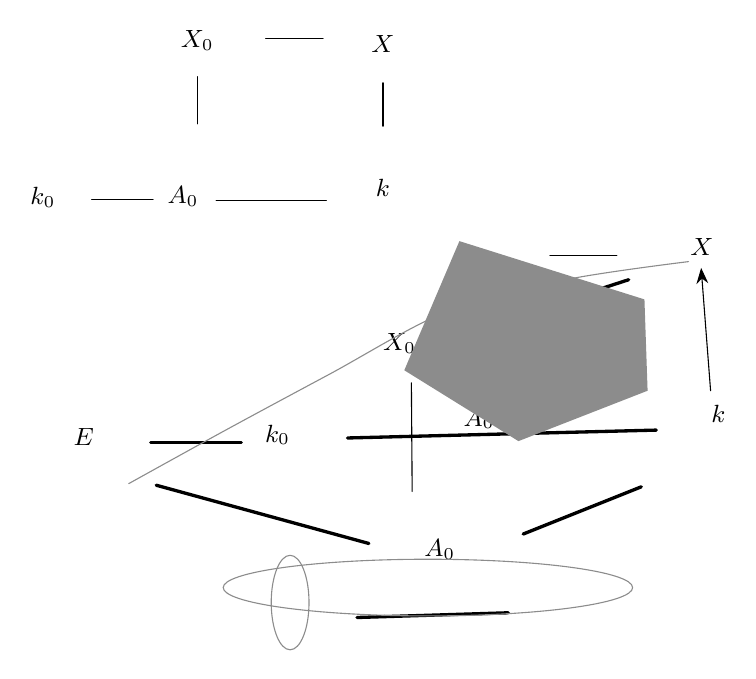
\begin{tikzpicture}[x=1mm,y=1mm,line cap=round,line join=round,font=\scriptsize]
\node[inner sep=1pt] at (28.2,-13.1) {\small $X_0$};
\draw (36.9,-12.9) -- (44.2,-12.9);
\node[inner sep=1pt] at (51.8,-13.6) {\small $X$};
\draw (28.2,-17.7) -- (28.2,-23.7);
\draw (51.8,-18.5) -- (51.8,-24);
\node[inner sep=1pt] at (8.6,-33) {\small $k_0$};
\draw (14.8,-33.3) -- (22.6,-33.3);
\node[inner sep=1pt] at (26.4,-32.9) {\small $A_0$};
\draw (30.6,-33.4) -- (44.6,-33.4);
\node[inner sep=1pt] at (51.8,-31.8) {\small $k$};
\node[inner sep=1pt] at (13.8,-63.5) {\small $E$};
\draw[very thick] (22.3,-64.2) -- (33.8,-64.2);
\node[inner sep=1pt] at (38.4,-63.2) {\small $k_0$};
\draw[very thick] (47.3,-63.6) -- (86.5,-62.6);
\node[inner sep=1pt] at (64,-61.2) {\small $A_0$};
\node[inner sep=1pt] at (53.9,-51.6) {\small $X_0$};
\draw (55.4,-56.6) -- (55.5,-70.4);
\draw[very thick] (65.4,-49.2) -- (83,-43.5);
\draw (73,-40.4) -- (81.5,-40.4);
\node[inner sep=1pt] at (92.3,-39.4) {\small $X$};
\draw[-{Stealth[length=2mm]}] (93.4,-57.6) -- (92.2,-42);
\node[inner sep=1pt] at (94.4,-60.6) {\small $k$};
\draw[very thick] (23,-69.6) -- (50,-77);
\node[inner sep=1pt] at (59,-77.8) {\small $A_0$};
\draw[very thick] (69.6,-75.8) -- (84.6,-69.8);
\draw[very thick] (48.5,-86.4) -- (67.7,-85.8);
\fill[pattern=north east lines,pencil] (54.5,-55) -- (61.5,-38.6) -- (85,-46) -- (85.4,-57.6) -- (69,-64) -- cycle;
\draw[pencil] plot[smooth, tension=0.55] coordinates {(19.5,-69.4) (32,-62.5) (45,-55.5) (60,-47.5) (75,-43.5) (90.6,-41.2)};
\draw[pencil] (57.5,-82.6) ellipse[x radius=26, y radius=3.6];
\draw[pencil] (40,-84.5) ellipse[x radius=2.4, y radius=6];
\end{tikzpicture}
\end{document}
